\documentclass{article}

\usepackage{graphicx}
\usepackage{multirow}
\usepackage{listings}
\usepackage{xcolor}
\usepackage[citecolor=black,linkcolor=black,urlcolor=blue,colorlinks=true]{hyperref}

\title{De novo Assembly of Second Generation Sequence Review}
\author{Sun Zhao\\zixiaojindao@gmail.com}

\begin{document}
\lstset{numbers=left,
numberstyle=\tiny,
keywordstyle=\color{blue!70}, commentstyle=\color{red!50!green!50!blue!50},
frame=shadowbox,
rulesepcolor=\color{red!20!green!20!blue!20}
}
\maketitle
\newpage

\begin{abstract}
Second-generation high-throughput sequencing methods generates large quantity short reads. Challenges including large scale input, exponential overlapping among reads, high possibility of repeat sequence make early methods based on ``overlap-layout-consensus" works badly. New methods depending on de bruijn graph approach succeed for short reads. This article presents the methods of the second generation sequencing, challenges for sequence assembly, how to assemble sequence in a pure computer science student's perspective. At last, my own contributions to sequence assembly are presented.
\end{abstract}

\section{Before Everything}
I would like to first explain the motivation of this article at the beginning. The theme of this article is about sequence assembly which is a computer aided process for constructing gene sequence. It is actually belonging to the scope of bioinformatics. As a pure computer science student, I have started researching in this field since the summer in 2010. After reading lots of papers, discussing with biology researchers from China as well as foreign ones, trying kinds of bioinformatic tools, I approached nothing new but valuable experiences of it. In this article, I will answer the questions of ``what is gene sequencing", ``what is sequence assembly and its challenge", ``how to assemble sequence", ``how to evaluate sequence assembly softwares" and my own contributions to sequence assembly in a computer science researcher's perspective. I'am not going to tell the deep details but giving initiations about what to do and how to do about sequence assembly. Moreover, I will provide valuable references of related papers and materials to help you get a full view of sequence assembly.
\section{What is gene sequencing}
In genetics and biochemistry, sequencing means to determine the primary structure of an unbranched biopolymer. The biopolymer can be DNA, RNA, protein. In this article, I will focus on DNA and RNA sequence analysis excluding protein. DNA sequencing is the process of determining the nucleotide order of a given DNA chain. Concretely, DNA is a chain of four types nucleotide, represented by letter of `A', `G', `C', `T'. DNA sequencing is trying to produce the corresponding string of `A', `G', `C', `T' for a sample DNA chain. However, the most popular biology sequencing method called shot gun, randomly cutting the original DNA chain into fragments and a set of `A', `G', `C', `T' strings. Each nucleotide string which is the sequence of a fragment is called a read. To increase the read coverage and read quality, copies of DNA made by PCR amplification with a typical bacteria template are sequenced. Fig. \ref{shot_gun_method} shows the shot gun process, and you may find that reads are sequenced from the two ends of DNA fragments instead of the complete one. The end sequencing phenomena is caused by biology sequencing methods, however, if particular reaction and methods are included, the distance between the two ends can be estimated. In this case, the two end reads are called pair-end reads and the distance is called insert length.\\
\begin{figure}[ht]
  \centering
  % Requires \usepackage{graphicx}
  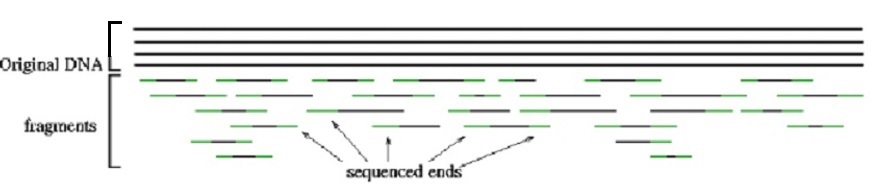
\includegraphics[width=8cm]{Figure1.jpg}\\
  \caption{}\label{shot_gun_method}
\end{figure}
DNA molecules are double-stranded helices, consisting of two long complement strands. According to base paring principle--`A' complements with `T' and `G' complements with `C', the sequence of a strand can be inferred from its opposite one. Particular sequences denoted by 3' and 5' in the DNA strand is used to specify the orientation of the two strand, and for simplicity, if one strand is specified as from 3' to 5', then the opposite one is from 5' to 3'. Example 1 shows a double strain DNA fragment with pair-end reads(red string). Note that the pair-end reads are positioned on opposite strand and will be sequenced all from 3' to 5'. So the two pair-end reads string should be `AGCTAA' and `GCCAA'.
\begin{center}
  3'$\rightarrow$5'\\
  {\color{red}AGCTAA}TGCTATCTTGGC\\
  TCGATTACGATAG{\color{red}AACCG}\\
  5'$\rightarrow$3'\\
  Example 1\\
\end{center}

\noindent Sequencing methods and platforms are developing as time goes. The typical genome analyser of first generation is Sanger\cite{sanger1977nucleotide} producing read lengths of approximately 800bp (typically 500-600bp with non-enriched DNA).Recently, new sequencing methods have emerged \cite{mardis2008impact}. Commercially available technologies include 454 Sequencing \cite{margulies2005genome}, Illumina genome analyser \cite{bentley2006whole} and SOLID sequencing(\href{www.appliedbiosystems.com}{www.appliedbiosystems.com}). Compared to traditional Sanger methods, these technologies function with significantly lower production costs and higher throughput. However, the reads produced by these next-generation sequencing technologies are much shorter than traditional Sanger reads, currently around 400-500 base pairs (bp) for 454, 50bp for Illumina and 35bp for SOLiD. Because of their length, they must be produced in large quantities and at greater coverage depths than earlier sequencing projects.\\
Reads are saved as a file by sequencing chip and the most popular format of read file is FASTA and FASTQ. A sequence in FASTA format begins with a single-line description, followed by lines of sequence data. The description line (def-line) is distinguished from the sequence data by a greater-than (``$>$") symbol at the beginning. It is recommended that all lines of text be shorter than 80 characters in length. An example sequence in FASTA format is shown in Fig. \ref{fasta_format}.A FASTQ file normally uses four lines per sequence. Line 1 begins with a '@' character and is followed by a sequence identifier and an optional description (like a FASTA title line). Line 2 is the raw sequence letters. Line 3 begins with a '+' character and is optionally followed by the same sequence identifier (and any description) again. Line 4 encodes the quality values for the sequence in Line 2, and must contain the same number of symbols as letters in the sequence. A minimal FASTQ file might look like Fig. \ref{fastq_format}. For more details about the quality line, please refer introduction on \href{http://en.wikipedia.org/wiki/FASTQ_format}{FASTQ Format}.\\
The last thing need to mention is RNA sequencing. As RNA is generated by transcription from DNA, the information is already present in the cell's DNA. The usual method to sequence RNA is first to reverse transcribe the sample to generate cDNA fragments. Then the cDNA are sequenced using DNA sequencing methods.\\
In a word, the next generation sequencing platform generates a FASTA/FASTQ format file consisting string of description, read and quality(only exists in FASTQ file) for DNA/RNA samples.
\begin{figure}[ht]
  \centering
  % Requires \usepackage{graphicx}
  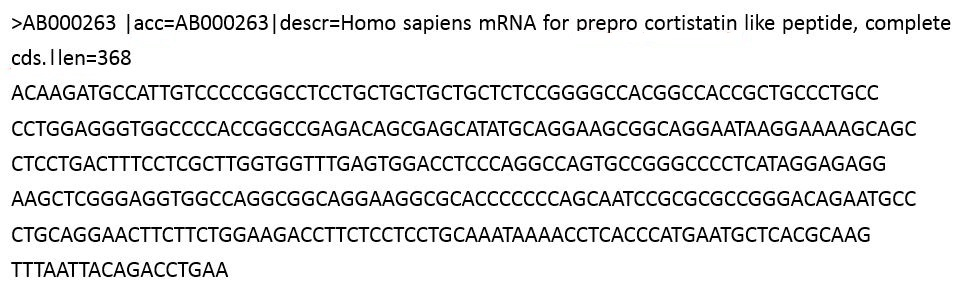
\includegraphics[width=10cm]{Figure2.jpg}\\
  \caption{}\label{fasta_format}
\end{figure}
\begin{figure}[ht]
  \centering
  % Requires \usepackage{graphicx}
  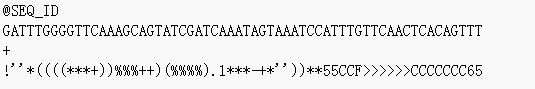
\includegraphics[width=10cm]{Figure3.jpg}\\
  \caption{}\label{fastq_format}
\end{figure}
\section{What is sequence assembly}
What the sequencing stage produces is a collection of DNA fragments's nucleotide sequence, whereas, what we need is the nucleotide sequence of the original one. Sequence assembly tries to align and merge the DNA fragments in order to reconstruct the original sequence. The intuition is to take advantage of overlap information between reads to tie them up and piece into a longer DNA sequence. Challenges listed blow makes sequence assembly a very complicated task.\\
\begin{itemize}
 \item One cell contains multiple chromosomes as well as DNA chains which are sequenced together. DNA fragments from different DNA chain may overlap each other.
 \item DNA is a double-stranded structure, one strand may overlap with its opposite one.
 \item Sheared fragments along the genome cannot be modeled as a perfect Poisson process so that there may be some region not covered by reads.
 \item DNA sequence may contains repeat regions, and these regions may be incorrectly merged by overlapping.
 \item Sequencing errors causes nucleotide deleting, replacing or inserting inside reads.
 \item Second generation sequencing platforms produce much shorter reads so that the overlapping possibility is exponentially increased.
\end{itemize}
Among those above challenges, the repeat problem is the most challenge thing for short read assembly. A simple example is shown in Fig. \ref{repeat_example}A, where the assembler incorrectly collapses the two copies of repeat A leading to the creation of two contigs instead of one Fig. \ref{repeat_example}B.\\
\begin{figure}[ht]
  \centering
  % Requires \usepackage{graphicx}
  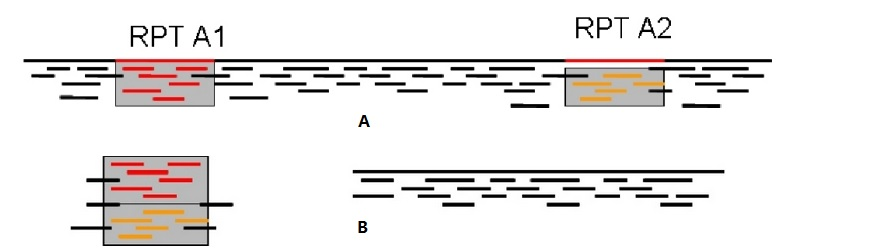
\includegraphics[width=10cm]{Figure4.jpg}\\
  \caption{}\label{repeat_example}
\end{figure}
\noindent The basic strategies for assembling sequences are categorized by two groups. One is reference based assembly, and the other one is de novo assembly. Reference based methods using a mapping tool to align reads against an existing reference sequence and build a sequence that is similar but not necessarily identical to the reference. The de novo assembly strategy does not use a reference sequence and is much useful for species whose reference sequence are unknown. This article only covers the de novo assembly and will illustrate the details in the subsequent sections.\\
Ideally, an assembly program should produce one contig for every chromosome of the genome being sequenced. However, because of challenge3 and challenge4, the output of the assembler is interrupted into a set of contigs. In summary, Inputting a FASTA/FASTQ read file, the assembler outputs a set of contigs.
\section{How to assembly sequence}
Overlap-consensus-layout \cite{myers1995toward} is the traditional approach for first generation sequence. It denotes each read as a separate node, where two reads presenting a clean overlap are connected by a bidirected edge. Although overlap-consensus-layout approach is both intuitive and robust, especially in the case of long reads, it is very costly for pair-wise overlap computing when assembling high quantity short reads produced by second generation sequencing platform like SOLID and Illumina. Only one microread assembler, EDENA \cite{hernandez2008novo} was developed using this approach. Later, Idury and Waterman \cite{idury1995new} introduced the use of a sequence graph to represent an assembly, and this idea has been developed into the most popular framework for short read assembly--De Bruijn graph. Sequence De Bruijn graph is constructed from a set of kmers(k is a parameter) as nodes, and two kmers are connected if one kmer's last k-1 nucleotides is identical to the first k-1 nucleotides. kmers are produced by moving a fixed length(k) sliding window on the original read. Examples of kmers and de bruijn graph are show in Fig. \ref{kmer_example} and Fig. \ref{debruijn_graph_example}. The sequence de bruijn graph has following properties:
\begin{itemize}
 \item Reads with length of n generates n-k+1 kmers.
 \item One read is mapping to a unique path in the de bruijn graph.
 \item One node has at most 4 successors and 4 predecessors by adding `A', `G', `C', `T' at the first or last of the k-1 nucleotides.
\end{itemize}
\begin{figure}[ht]
  \centering
  % Requires \usepackage{graphicx}
  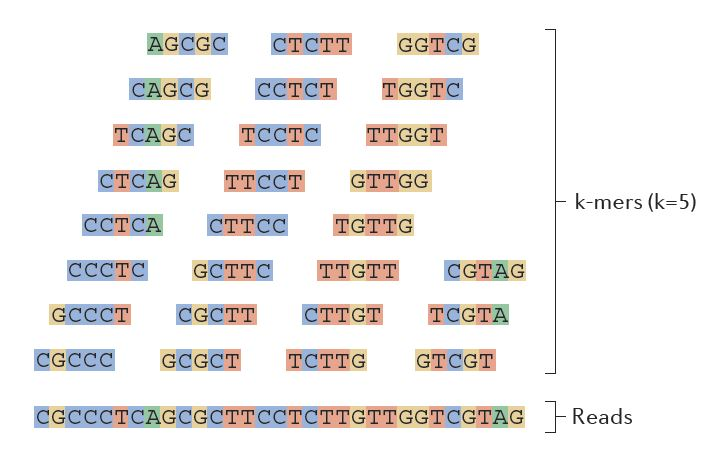
\includegraphics[width=10cm]{Figure5.jpg}\\
  \caption{}\label{kmer_example}
\end{figure}
\begin{figure}[ht]
  \centering
  % Requires \usepackage{graphicx}
  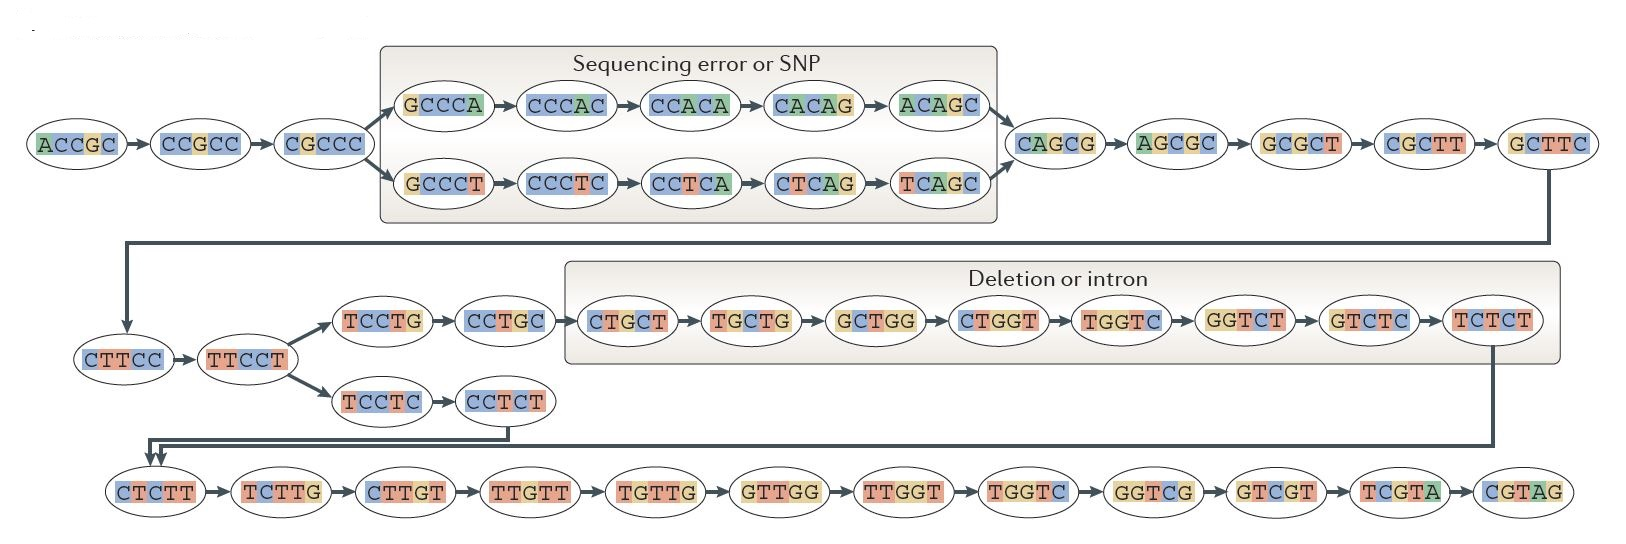
\includegraphics[width=10cm]{Figure6.jpg}\\
  \caption{}\label{debruijn_graph_example}
\end{figure}
According the property2 and property3, the node scale of the de bruijn graph is bounded by O(n-k+1) and the edge scale of it is bounded by O(8(n-k+1)) where n is the length of target origin DNA sequence. By the way, the length of human genome is about 3G base pairs whose de bruijn graph can be stored in a single server machine or cluster configured with 128GB. Property3 releases the heavy cost of searching for all pair-wise overlap, thus making de bruijn graph approach feasible. Softwares include Velvet \cite{zerbino2008velvet}, ABYSS \cite{simpson2009abyss}, ALLPATHS \cite{butler2008allpaths}, SOAPDenovo \cite{li2010novo} follows the de bruijn graph method. ABYSS and ALLPATHS claimed that they successfully assembled human's genome. A brief comparison of these softwares is show in Table \ref{comparison_of_assemblers}. Software links can be found in Table \ref{links_of_assemblers}.\\
I've read code and run programs of Velvet and ABYSS and provide some details about them. Velvet consists of two modules named velveth and velvetg where `h' means hash and `g' means graph. Velvet designed a novel graph construction algorithm and claim that it is efficient and memory saving approach on a single machine. velveth sequentially reads the FASTA/FASTQ read file and for each k-mer observed in the set of reads, a hash table records the ID of the first read encountered containing that k-mer and the position of its occurrence within that read. Each k-mer is recorded simultaneously to its reverse complement sequence. To ensure that each k-mer cannot be its own reverse complement, k must be odd. This first scan allows each read to be re-written as a set of new k-mers combined to overlaps with previously hashed reads. This new representation of the reads sequence is called a roadmap which is written into a file named ROADMAP. velvetg reads the ROADMAP file and creats a second database with the opposite information. It records, for each read, which of its original k-mers are overlapped by subsequent reads. The ordered set of original k-mers of that read is cut each time an overlap with another read begins or ends. For each uninterrupted sequence of original k-mers, a node is created. Finally, reads are traced through the graph using the roadmaps. Knowing the correspondence between original k-mers and the newly created nodes, it is possible to proceed from one node to the next, creating a new directed arc or incrementing the multiplicity of an existing one as appropriate at each step. The final output of velvet is produced by velvetg and saved as config.fa. ABYSS constructs de bruijn graph directly following the definition. The MPI version uses a hash function to determine the host machine for a node. The structure of ABYSS program is organized by a make file driver named ``abyss-pe". abyss-pe automatically finds the dependency of abyss modules and perform a minimum number of running modules. The final output is saved as *-contigs.fa, *-scanffolds.fa, *-unitigs.fa and a statistic file named *-stats.\\
\begin{table}[ht]
\begin{center}
\caption{}\label{comparison_of_assemblers}
\begin{tabular}{c|c|c|c}
\hline
Software & Parallelism & Large Scale Assembly & Memory Cost\\
\hline
Velvet & OpenMP & No & High\\
\hline
ABYSS & OpenMP+MPI & Yes & Low\\
\hline
ALLPATH& ? & Yes & ?\\
\hline
SOAPDenovo & ? & Yes &Low\\
\hline
\end{tabular}
\end{center}
\end{table}
\begin{table}[ht]
\begin{center}
\caption{}\label{links_of_assemblers}
\begin{tabular}{l|l}
\hline
Software &Software Available\\
\hline
Velvet &\href{http://www.ebi.ac.uk/~zerbino/velvet/}{http://www.ebi.ac.uk/~zerbino/velvet/}\\
\hline
ABYSS &\href{http://www.bcgsc.ca/platform/bioinfo/software/abyss/}{http://www.bcgsc.ca/platform/bioinfo/software/abyss/}\\
\hline
ALLPATH &\href{http://www.broadinstitute.org/science/programs/genome-biology/crd}{http://www.broadinstitute.org/science/programs/genome-biology/crd}\\
\hline
SOAPDenovo &\href{http://soap.genomics.org.cn/soapdenovo.html}{http://soap.genomics.org.cn/soapdenovo.html}\\
\hline
\end{tabular}
\end{center}
\end{table}
\noindent After building the de bruijn graph, a graph correction process is applied. The idea of the graph correction process is to simplify the original graph into a long path by removing branches. There are two types of branches--tips and bubbles. A tip is a chain of nodes which is disconnected on one end and a bubble is a circle with two common end points. Whenever a node A has only one outgoing arc that points to another node B that has only one incoming arc, the two nodes can be merged into a long node. Tips and bubbles are shown in Fig .\ref{branch_example}. Note that repeat regions also create circles in the graph, and we can not determine how many times does the repeat sequence occur. In the last step, if pair-end reads are provided, we can estimate the distance of seed nodes and find a feasible path between them.\\
The last thing need to mention is that RNA assembly also named transcript assembly. RNA assembly is more complex than DNA assembly, observing the reasons:
\begin{itemize}
 \item Some transcripts have low coverage, whereas others are highly expressed.
 \item Reads with sequencing errors derived from a highly expressed transcript may be more abundant than correct reads from a transcript that is not highly expressed.
 \item Transcripts encoded by adjacent loci can overlap and thus can be erroneously fused to form a chimeric transcript.
\end{itemize}
Directly using DNA assemblers to assemble RNA sequences only outputs rather bad results. Velvet and ABYSS have extend themselves into Velvet\_Oases \cite{schulz2012oases} and Trans-ABYSS \cite{robertson2010novo} separately to address the additional challenges presented by RNA assembly. Recently, Trinity \cite{grabherr2011full} was specially designed for transcript assembly. Zhao et. al \cite{zhao2011optimizing} made an early comparison of transcript assembly and give a full view of performance, result, resource usage evaluation. It shows Trinity has a relative better assembling ability than Velvet\_Oases and Trans-ABYSS but much slower and memory cost while assembling large scale sequences. A group of HPC developers \cite{henschel2012trinity} made efforts to accelerating Trinity and reducing its memory usage which make trinity a first choice when assembling transcript sequences.
\begin{figure}[ht]
  \centering
  % Requires \usepackage{graphicx}
  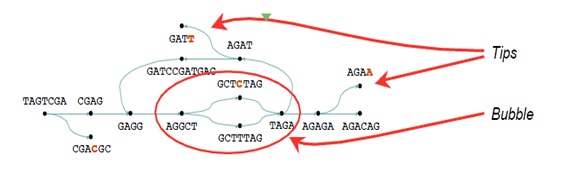
\includegraphics[width=10cm]{Figure7.jpg}\\
  \caption{}\label{branch_example}
\end{figure}
\section{How to Evaluate Assembler}
To evaluate present assemblers or assemblers designed by ourselves, the first thing to do is to prepare input data. Usually, two kinds of data are used to evaluate assemblers, synthetic data and real data. dwgsim \footnote{http://sourceforge.net/apps/mediawiki/dnaa/index.php?title=Whole\_Genome\_Simulation} is a whole genome simulator based on a reference genome. Reference genome can be found on \href{ftp://ftp.ncbi.nlm.nih.gov/refseq/}{ftp://ftp.ncbi.nlm.nih.gov/refseq/}, \href{ftp://ftp.ncbi.nlm.nih.gov/genomes/}{ftp://ftp.ncbi.nlm.nih.gov/genomes/} or NCBI's nucleotide database (\href{http://www.ncbi.nlm.nih.gov/nucleotide}{http://www.ncbi.nlm.nih.gov/nucleotide}). Details about refseq is explained on \href{http://www.ncbi.nlm.nih.gov/books/NBK50679/}{http://www.ncbi.nlm.nih.gov/books/NBK50679/}. NCBI's SRA database \footnote{http://www.ncbi.nlm.nih.gov/sra} provides a large collection of read sequences. Users search this database using an access code begin with SRP(studies), SRS(samples), SRX(experients) or SRR(runs). Multiple SRRs of same samples can be used together as input. By the way, files downloaded from SRA database are in sra format and users should dump out FASTA/FASTQ format using fastq-dump from \href{http://trace.ncbi.nlm.nih.gov/Traces/sra/sra.cgi?view=software}{NCBI SRA Toolkit}. If pair-end data are expected to be dumped, pass `--split-3' or `--split-files' to fastq-dump. Metrics for evaluate assembler can be N50 length, running time, memory cost, 95\% map ratio and so on. Given a set of contigs(output of assemblers) of varying lengths, the N50 length is defined as the length N for which half of all bases in the sequences are in a sequence of length L $<$ N. Obviously, the larger the N50 length, the better the assembled contigs. On linux like systems, users can use `/usr/bin/time -v' command to record the running time and peak memory usage of a user process. The 95\% mapping ratio is defined as the number of contigs with at least 95\% identity mapping to the reference dividing by the total number of contigs. BLAST \cite{altschul1990basic} and BLAT \cite{kent2002blat} are two popular mapping tools for aligning contigs to references. I often choose BLAT for reasons of efficiency. BLAT outputs a very big table(PSL format) to store the mapping info for each query sequence. Users who are strange to PSL format and the meaning of each column should refer to \href{http://genome.ucsc.edu/FAQ/FAQformat.html#format2}{PSL format}. Each query may have multiple candidate alignment positions, and BLAT program doesn't provide a percent identity value column or score column like the web BLAT \footnote{http://www.genoscope.cns.fr/blat-server/cgi-bin/vitis/webBlat}. Users can replicate the two columns referring to \href{http://www.genoscope.cns.fr/blat-server/cgi-bin/vitis/webBlat}{http://www.genoscope.cns.fr/blat-server/cgi-bin/vitis/webBlat} and use the best hit to calculate 95\% mapping ratio.
\section{My Own Contribution}
My own contributions to the sequence assembly are shown in Table \ref{my_own_contribution}.
\begin{table}[ht]
\begin{center}
\caption{}\label{my_own_contribution}
\begin{tabular}{l|l}
\hline
Contribution &Links\\
\hline
Velvet and Oases for windows&\href{https://github.com/zixiaojindao/velvet.git}{https://github.com/zixiaojindao/velvet.git}\\
\hline
ABYSS for windows &\href{https://github.com/zixiaojindao/ABYSS.git}{https://github.com/zixiaojindao/ABYSS.git}\\
\hline
MemoryUsageMonitor for windows &\href{https://github.com/zixiaojindao/MemoryUsageMonitor.git}{https://github.com/zixiaojindao/MemoryUsageMonitor.git}\\
\hline
blat-statistics for windows &\href{https://github.com/zixiaojindao/blat-statistics.git}{https://github.com/zixiaojindao/blat-statistics.git}\\
\hline
Sequence Assembly Information & \href{https://github.com/zixiaojindao/RNA-sequence-info.git}{https://github.com/zixiaojindao/RNA-sequence-info.git}\\
\hline
\end{tabular}
\end{center}
\end{table}
\section{Tutorial of Tools}
This section describes a concrete example covering preparing synthetic data, using Velvet and ABYSS and evaluating result. Synthetic read data are generated by `dwgsim' inputting a reference sequence. We choose yeast data and download reference sequence named chrosome1.fasta, chrosome2.fasta chrosome3.fasta separately at \href{ftp://ftp.sanger.ac.uk/pub2/yeast/pombe/Chromosome\_contigs/}{ftp://ftp.sanger.ac.uk/pub2/yeast/pombe/Chromosome\_contigs/}.
\begin{lstlisting}
dwgsim -N 1000000 chrosome1.fasta c1
\end{lstlisting}
Above command generates 1000000 pair-end reads saved as c1.bwa.read1.fastq and c1.bwa.read2.fastq. These two files are the raw input for assemblers. Next we need compile Velvet for windows and ABYSS for windows. Velvet for windows is ported by visual studio 2012. Please make sure that all the projects are configured with x64 platform after opening the solution, and release version is preferable. When finishing building the solution, velveth.exe, velvetg.exe and oases.exe should be found in the \emph{bin} directory. Then type
\begin{lstlisting}
velveth tt1 25 -fastq -shortPaired c1.bwa.read.fastq
velvetg tt1 -ins_length 500 -exp_cov auto
\end{lstlisting}
This will force Velvet working and producing the final assembled result. More details about the usage of velvet, please refer to the manual pdf in the source.\\
Considering ABYSS for windows, \href{http://downloads.sourceforge.net/project/boost/boost/1.49.0/boost_1_49_0.tar.bz2}{boost1.49} should be downloaded and uncompressed in the source directory. Configure ABYSS with x64 platform in visual studio 2012 and build all the projects and you will get all the binaries in the \emph{bin} directory. Note that ABYSS uses a make file driver as user interface, users have to use a linux bash like cygwin to run it. You might use following commands to assemble our synthetic data:
\begin{lstlisting}
time abyss-pe name=tt k=25 in=`c1.bwa.read1.fastq\
c1.bwa.read2.fastq' | tee tt.output
\end{lstlisting}
ABYSS for windows uses \href{http://www.microsoft.com/zh-cn/download/details.aspx?id=14737}{microsoft MPI package} as mpi library. To use mpi version, just add `np' option to `abyss-pe' like
\begin{lstlisting}
time abyss-pe np=4 name=tt k=25 in=`c1.bwa.read1.fastq\
c1.bwa.read2.fastq' | tee tt.output
\end{lstlisting}
More details about ABYSS, please refer to the ReadMe.html in the source directory or \href{https://github.com/sjackman/abyss}{ABYSS origin}.\\
Metrics for evaluate assembler are N50 length, running time, memory cost and 95\% map ratio. N50 as well as NX0 is calculated and printed by Velvet and ABYSS themselves. On windows, I create a resource monitor tool mentioned in the contribution section, and feel free to use other alternatives. BLAT is used to align contigs to reference and calculate 95\% map ratio. Following the yeast example, we evaluate Velvet's result named contigs.fa in \emph{tt1} directory. Users may type
\begin{lstlisting}
blat chrosome1.fasta contigs.fa blat.output
blat-statistics blat.output.psl chrosome1.fasta contigs.fa
\end{lstlisting}
blat-statistics is a tool used to parse PSL file produced by BLAT and calculate some statistics about it. blat-statistics is originally developed on windows using C++ and additional efforts are need to compile it on linux.
\section{Summary}
In a programmer's perspective, sequence assembly is piecing string fragments into a set of long strings using overlap among them. However, things are much complicated in practice due to biological challenges. Most of assembly softwares follow the de bruijn graph approach and reach a satisfying point. However, the running time and memory cost for large scale sequence is still not very good as well as assembled contigs. Hope new computer algorithms and biological methods could help address this problem much better in the future.
\renewcommand\refname{Reference}
\bibliographystyle{plain}
\bibliography{Thesis}
\end{document}
